\documentclass[12pt, titlepage]{article}
\usepackage[a4paper, nomarginpar, total={210mm,297mm}, left=25mm, right=15mm, top=20mm, bottom=20mm]{geometry}

\title{Elektroninės prekybos situacija Lietuvoje per paskutinius 5 metus}
\author{Rokas Krupinskas}

\usepackage[utf8]{inputenc}
\usepackage[L7x]{fontenc}
\usepackage[lithuanian]{babel}
\usepackage{tgtermes}
\usepackage{graphicx}
\usepackage{float}

\usepackage{setspace}
\onehalfspacing
\usepackage{hyperref}
\hypersetup{
	colorlinks=true,
	linkcolor=black,
	filecolor=blue,
	urlcolor=blue,
	citecolor=black}

\usepackage[
backend=biber,
style=apa,
url=false,
sorting=nyt]{biblatex}
\setlength{\parindent}{4em}

\addbibresource{lit.bib}

\begin{document}
\maketitle
\tableofcontents
\newpage

\section{Įvadas}
\smallskip
\par
\hspace{\parindent}
Informacinės ir komunikacinės technologijos dvidešimt pirmajame amžiuje skverbiasi į visas veiklos sritis. Žmonių veikla darosi nepriklausoma nuo atstumų tarp jų, technologijos tampa įprastine, kasdienine žmonių aplinka.( \textcite{davidavivciene2011elektronines}) Šiuolaikinėje visuomenėje nekyla klausimas, ar būti internete, tai tampa būtinybe. Anot \cite{benesevivciene2014veiksniku}, internetas tampa ne tik informacijos, bendravimo, žinių pasikeitimo, bet ir verslo vystymo terpe. Vis daugiau įmonių savo veiklą plečia ne geografinio regiono aspektu internete ir dėl spartaus interneto ryšio paplitimo internetas tapo ne vien svarbus kasdieniniame gyvenime, bet ir versle. Sparčiai besivystančių informacinių technologijų pasekoje, atsirado naujos ekonominės formos, tarp jų ir internetinė prekyba (\textcite{dambrauskaite2014elektronines}).
\par
Pagal Lietuvos statistikos departamento (LSD) duomenis namų ūkių, turinčių interneto prieigą skaičius, per 2014 - 2018 metus padaugėjo nuo 66 iki 78.4 procentų (žiūrėti pav nr. \ref{fig:2}). Nors ir Lietuva anksčiau atsiliko nuo kitų Europos šalių šiuo aspektu, tačiau iš \ref{fig:1} grafiko galima pamatyti, jog Lietuvoje per paskutinius 5 metus interneto prieiga namų ūkiuose augo greičiau nei EU28 šalyse.
\par
Taip pat dėl palankių techninių sąlygų žymiai padidėjo elektroninės prekybos svetainių skaičius Lietuvoje. Remiantis www.eshops.lt duomenimis, 2011m. vasario mėnesį Lietuvoje buvo 985 elektroninės parduotuvės, o jau 2018m. birželio mėnesį -  net 2331 (\textcite{vsivickas2011elektronine}). Pasak \textcite{davidavivciene2011elektronines}, vienas iš populiariausių būdų konkuruoti informacinių technologijų amžiuje – interneto svetainės, kurios vis plačiau naudojamos komerciniais tikslais. Tačiau perkeliant dalį asmeninio verslo į internetą, nėra garantuojamas pranašumas prieš kitas firmas ir įmones, prekiaujančias internetu, nes atsiranda galimybė pasirinkti iš be galo daug labai panašių svetainių. Kaip teigia \cite{pabedinskaite2012vartotojku}, elektroninei prekybai Lietuvoje kaip ir kitose šalyse kyla iššūkiai, nes vartotojų elgsena internete skiriasi nuo elgsenos tradicinėje prekyboje, todėl Lietuvoje dalis vartotojų nepasitiki elektronine prekyba ir teikia pirmenybę tradicinei. Nuolatos besivystančių ir viena kita keičiančių informacinių technologijų amžiuje, elektroninėje erdvėje naudojama informacija apie individus tampa vertinga preke ir tai lemia elektroninės prekybos sparčiausią augimą tarp visų verslo sektorių.
\smallskip
\par
\noindent
Darbo tikslas: atskleisti elektroninės prekybos situaciją Lietuvoje per paskutinius 5 metus.
\smallskip
\par
\noindent
Darbo uždaviniai:
\begin{enumerate}
\item Išsiaiškinti kokie yra teigiami ir neigiami elektroninės prekybos aspektai.
\item Aptarti internetinės prekybos prekėmis ir paslaugomis plėtrą Lietuvoje 2014-2018 m.
\end{enumerate}
\newpage
\section{Elektroninės prekybos privalumai ir trūkumai}
\subsection{Privalumai}
\smallskip
\par
\hspace{\parindent}
Elektroninė prekyba prekėmis ir paslaugomis internetu turi teigiamų ir neigiamų aspektų ir daro įtaką vartotojo elgsenai bei sprendimui įsigyti prekių ir paslaugų internetu. Informacinės plėtros komitetas pabrėžia tokius elektroninės prekybos privalumus: (nuoroda į Informacinės visuomenės plėtros komitetą: \href{https://ivpk.lrv.lt} {Ivpk})
\smallskip
\begin{enumerate}
\item Paprasta ir greita – tereikia jaukiai įsitaisyti priešais monitorių, keletą kartų spustelti pelės ir klaviatūros klavišus – dėl prekės pirkimo ir pristatymo ar paslaugos suteikimo bus susitarta.
\item Patogu – nėra būtinybės vykti į pardavėjo veiklos vietą, kuri gali būti tiek kitame mieste, tiek kitoje pasaulio pusėje, nereikia derintis prie pardavėjo darbo valandų.
\item Pigu – dažnai internete veikiančių asmenų siūlomų įsigyti prekių ar paslaugų kaina būna kur kas mažesnė, nei asmenų, veiklą vykdančių konkrečiu fiziniu adresu.
\item Informatyvu – galimybė rasti daug ir išsamios informacijos apie siūlomas prekes/paslaugas ir jų pardavėjus.
\item Asortimento apimtis – internetu pasiekiama nepalyginamai didesnė prekių ir paslaugų įvairovė nei lokalioje rinkoje.
\item Papildoma pirkėjo teisių apsauga – teisė per 7 darbo dienas nenurodant priežasčių grąžinti nepatikusias prekes ar atsisakyti paslaugų ir atgauti visus sumokėtus pinigus.
\end{enumerate}
\medskip
\par
Panašius privalumus pamini ir kiti autoriai, savo darbuose nagrinėję elektroninę komerciją ir jos aspektus. Remiantis \textcite{dambrauskaite2014elektronines}, galima išskirti šiuos privalumus: prekyba internetu padeda taupyti laiką vykdant atsiskaitymus, panaudojami ištekliai ir sąnaudos yra mažesnės nei tradicinėje prekyboje, galima įsigyti prekių iš bet kur, tiesiogiai iš gamintojo, geresnis ir greitesnis klientų aptarnavimas, lemiantis didesnį produktyvumo ir efektyvumo lygį. Pasak \textcite{bernotavivciute2013produktku}, vienas iš daugelio privalumų yra tai, jog perkant internetinėje erdvėje nėra šalia stovinčių pardavėjų, kurie bandytų įsiūlyti parduodamą prekę ir įkalbinėti įsigyti kitų prekių ar paslaugų ar pamėginti naują produktą, kaip dažnai atsitinka prekybos centruose.
Tuo tarpu \textcite{jurgelionyte2010elektronines} teigia, jog svarbiausias elektroninių parduotuvių privalumas – galimybė palyginti kelių parduotuvių kainas vienu metu ir pirkti prekes, neišeinant iš namų.  Taip pat minimas platesnis prekių asortimentas, mažesnės kainos ir eilių nebuvimas ir labai dažnas veikimas visą parą.
\medskip
\subsection{Trūkumai}
\smallskip
\par
\hspace{\parindent}
Nors ir prekyba internetu turi nemažai privalumų, tačiau ji turi ir trūkumų, kurie neretai ir yra priežastys, kodėl asmenys nusprendžia nepirkti elektroninėje erdvėje. Informacinės plėtros komitetas nurodo tokius elektroninės prekybos trūkumus - rizikas: (nuoroda į Informacinės visuomenės plėtros komitetą: \href{https://ivpk.lrv.lt} {Ivpk})
\smallskip
\begin{enumerate}
\item Įsigyta prekė gali būti neatsiųsta ar paslauga nesuteikta.
\item Gali būti atsiųsta ar suteikta netinkamos kokybės prekė ar paslauga, o pardavėjas gali nesutikti grąžinti sumokėtą kainą/pakeisti netinkamą prekę tinkama, ar su pardavėju apskritai gali nepavykti susisiekti.
\item Gali būti tiek teisėtu būdu įgyjama (pvz., pildant sandorio sudarymui būtinus dokumentus), tiek ir neteisėtu būtu įgyjama (pvz., išviliojama prisidengiant išgalvotomis istorijomis ar pavagiama pasinaudojant šnipinėjimui skirta programine įranga) pirkėjo asmeninė informacija (įskaitant finansinę informaciją, privačius duomenis) bei panaudojama neteisėtais tikslais.
\end{enumerate}
\smallskip
\par
Kiti autoriai išskiria panašius, bet taip pat ir skirtingus trūkumus. \textcite{dambrauskaite2014elektronines} teigimu, saugumo trūkumas, neegzistuojanti galimybė paliesti ir pajusti fiziškai prekės, internetiniai trukdžiai ir trūkstama prieiga prie interneto arba kompiuterio, taip pat sudėtingi muitai, perkant iš užsienio svetainių ir persiuntimo išlaidos. \textcite{jurgelionyte2010elektronines} akcentuoja šiuos trūkumus, stabdančius elektroninę prekybą: dažnas vartotojų nepasitikėjimas ir virtualios edvės siejimas su rizika ir techninėmis problemomis, abejonės, atsirandančios dėl trūkstamos informacijos apie internetinės prekybos galimybes ar prašymu pateikti per daug asmeninės informacijos, kuri gal net ir nebūtina. Tuo pačiu vartotojas dažnai nesirenka elektroninės prekybos, nes negali įvertinti prekės kokybės ir nepatiria momentinio apsipirkimo džiaugsmo. Tuo tarpu \textcite{vsivickas2011elektronine} irgi pabrėžia, kad pirkėjas susilaiko nuo pirkimo internetu, nes negali įvertinti prekės kokybės, o tai yra vienas iš pagrindinių informacijos apie prekę išgavimo būdų ir nemažai atvejų yra lemiamas motyvas pirkti. Antra, nors ir tradicinėje prekyboje pasitaiko neoriginalios prekės, tačiau internetinėje prekyboje yra žymiai sudėtingiau atskirti originalų nuo neoriginalaus daikto ir patikimą informaciją nuo nepatikimos. Taip pat pasak autoriaus, vėliau gautas užsakytas pirkinys gali skirtis nuo to, ko tikėjosi vartotojas pirkdamas internetu ir dar vienas trūkumas internetinės prekybos yra laikas, tenkantis pristatyti prekę ar paslaugą, kitaip nei tradicinėje prekyboje, kur toje pačioje vietoje galima įsigyti iš karto.
Tai patvirtina ir Eurostat pateikiami duomenys apie problemas, su kuriomis susiduria elektroninės prekybos klientai ir priežastys, nulemenčios pasirinkimą neįsigyti prekių ir paslaugų internetu (žiūrėti lenteles nr. \ref{tab:2} ir \ref{tab:1}).
\medskip
\begin{table}[H]
\centering
\caption{Priežastys nepirkimui internetu, EU28 (\% asmenų, kurie nepirko ir neužsisakė prekių ar paslaugų per internetą
privačiam naudojimui per paskutinius 12 mėnesių)
Šaltinis: sudaryta autoriaus, remiantis Eurostat (isoc\_ec\_inb)}
\label{tab:2}
\begin{tabular}{|l|c|}
\hline
\multicolumn{1}{|c|}{Priežastis}                                                                                                      & Procentai \\ \hline
\begin{tabular}[c]{@{}l@{}}Neturi mokėjimui internetu\\ skirtos kortelės\end{tabular}                                                 & 12        \\ \hline
\begin{tabular}[c]{@{}l@{}}Abejonės dėl apmokėjimo \\ saugumo\end{tabular}                                                            & 25        \\ \hline
\begin{tabular}[c]{@{}l@{}}Teikia pirmenybę apsipirkimui \\ gyvai, nori matyti prekę ir tai įprastas\\ apsipirkimo būdas\end{tabular} & 69        \\ \hline
Trūksta reikiamų įgūdžių                                                                                                              & 19        \\ \hline
Pristatymas prekių yra problema                                                                                                       & 6         \\ \hline
\begin{tabular}[c]{@{}l@{}}Papildomi rūpesčiai dėl grąžinimo arba gavimo\\ prekių, skundų/žalos atlyginimo\end{tabular}               & 19        \\ \hline
\end{tabular}
\end{table}
\bigskip
\begin{table}[H]
\centering
\caption{Problemos, su kuriomis susidurta perkant internetu EU28, 2017m. (\% of asmenų, kurie pirko arba užsisakė prekių arba paslaugų privačiam naudojimui per paskutinius 12 mėnesių)
Šaltinis: sudaryta autoriaus, remiantis Eurostat (isoc\_ec\_iprb)}
\label{tab:1}
\medskip
\begin{tabular}{|c|c|c|}
\hline
Metai & Problema                                                                                & Procentai \\ \hline
2017  & Nebuvo jokių problemų                                                                   & 69        \\ \hline
2017  & \begin{tabular}[c]{@{}c@{}}Užsienio mažmenininkas\\ neparduoda mano šalyje\end{tabular} & 3         \\ \hline
2017  & Apgavystė                                                                               & 3         \\ \hline
2017  & \begin{tabular}[c]{@{}c@{}}Pristatymas užtruko ilgiau\\ nei nurodyta\end{tabular}       & 17        \\ \hline
2017  & Techninis gedimas                                                                       & 11        \\ \hline
\end{tabular}
\centering
\end{table}
\medskip
\subsection{Apibendrinimas}
\smallskip
\par
\hspace{\parindent}
Kaip pastebi \textcite{dambrauskaite2014elektronines}, elektroninė komercija padeda pateikti savo siūlomą prekę ar paslaugą didesniam kiekiui asmenų ir pritraukti didesnį vartotojų skaičių nei tradicinė prekyba. Elektroninės prekybos plėtra garantuoja potencialių darbo vietų atsiradimą, todėl elektroninė komercija yra be galo svarbi kiekvienos šalies ekonomikai, tačiau elektroninės prekybos prekėmis ir paslaugomis privalumai ir trūkumai lemia vartotojų apsispredimą įsigyti prekių ir paslaugų internete ir tuo pačiu internetinės prekybos plėtrą. 
\newpage
\section{Plėtra}
\smallskip
\par
\hspace{\parindent}
Elektroninės prekybos prekėmis ir paslaugomis plėtrai gali turėti įtakos daugelis veiksnių, todėl internetinė prekyba nevienodai sparčiai vystėsi visame pasaulyje, taip pat ir Europos regione. Pagal Eurostat duomenis (žiūrėti lentelę nr. \ref{tab:3}) galima teigti, kad per paskutinius 5 metus asmenų, kurie pirko internetu skaičius Lietuvoje išaugo beveik 1.5 karto, o Europos 28 šalių vidurkis padidėjo nežymiai. Kaip pastebi \textcite{klapatauskiene2013elektronines}, Lietuvoje elektroninės komercijos plėtrai teigiamą įtaką turi informacinių ir telekomunikacinių technologijų plėtra, užsienio įmonių investicijos bei nemažas interneto ir kitas programavimo paslaugas teikiančių įmonių skaičius. 
\medskip
\begin{figure}[H]
\center
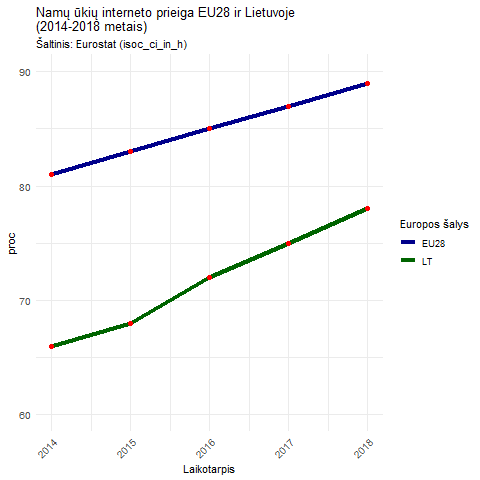
\includegraphics[scale=0.9]{Grafikai/4.png} 
\caption{Grafikas 1}
\label{fig:1}
\end{figure}
\bigskip
\begin{figure}[H]
\center
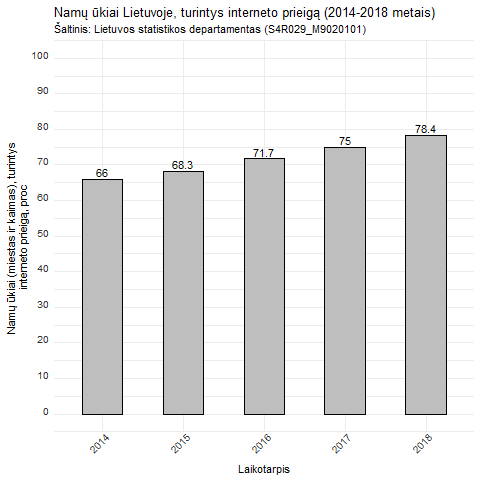
\includegraphics[scale=0.8]{Grafikai/1.png} 
\caption{Grafikas 2}
\label{fig:2}
\end{figure}
\bigskip
Nuoroda į Lietuvos statistikos departamentą: \href{https://osp.stat.gov.lt/}{LSD}
\medskip
\begin{table}[H]
\centering
\caption{Procentai visų asmenų, besinaudojusių internetu per paskutinius metus, kurie pirko internetu per paskutinius 12 mėnesių Lietuvoje ir EU28 (2014 - 2018 metais)
Šaltinis:sudaryta autoriaus, remiantis Eurostat (isoc\_ec\_ibuy)}
\label{tab:3}
\begin{tabular}{|l|c|c|c|l|l|l|}
\hline
  & Europos šalis & Laikotarpis & \multicolumn{1}{r|}{Procentai} & Europos šalis & Laikotarpis & Procentai \\ \hline
1 & EU28          & 2014        & 63                             & LT            & 2014        & 36        \\ \hline
2 & EU28          & 2015        & 65                             & LT            & 2015        & 44        \\ \hline
3 & EU28          & 2016        & 66                             & LT            & 2016        & 44        \\ \hline
4 & EU28          & 2017        & 68                             & LT            & 2017        & 49        \\ \hline
5 & EU28          & 2018        & 69                             & LT            & 2018        & 54        \\
\hline
\end{tabular}
\end{table}
\smallskip
\par
\textcite{pabedinskaite2012vartotojku} išskiria išorinius aplinkos veiksnius, kurie lemia elektroninės prekybos plėtrą šalyje t.y technines galimybes, kitaip tariant kompiuterių ir interneto paplitimas šalyje ir kiti išorinės aplinkos veiksniai. Tai patvirtina Lietuvos statistikos duomenys (žiūrėti pav nr. \ref{fig:2}) ir Eurostat duomenys (žiūrėti pav nr. \ref{fig:1}), kurie leidžia daryti išvadą, jog Lietuvoje, gerėjančios technologinės galimybės turėjo įtakos sėkmingai elektroninės prekybos plėtrai. Pagal naudojimąsi internetine prekyba 2018 metais (žiūrėti pav nr. \ref{fig:4}), aktyviausi yra 25-34 metų asmenys (58.5 procentai), antroje vietoje yra 16-29 metų asmenys (54 procentai). Trečioje vietoje yra 35-44 metų asmenys, pralenkę 16-24 metų amžiaus grupę 0.1 procentu, o iš vyresniojo amžiaus gyventojų (65-74 metų) elektronine prekyba naudojosi 5.1 procento. Taigi didžioji dalis besinaudojančių internetine prekyba yra jauni žmonės. Taip pat šiame grafike galima pastebėti tendenciją, jog per pastaruosius metus elektroninė prekyba Lietuvoje išaugo tarp visų amžiaus grupių.
\begin{figure}[H]
\center
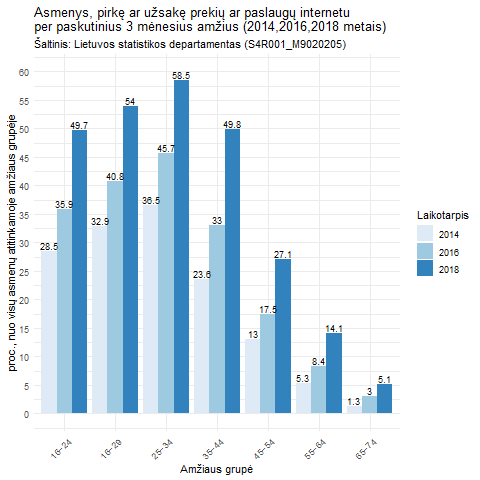
\includegraphics[scale=0.8]{Grafikai/3.png} 
\caption{Grafikas 3}
\label{fig:4}
\end{figure}
\medskip
\par
Lyginant 2014 ir 2018 metų duomenis (žiūrėti į pav nr. \ref{fig:5}), 2018 metais Lietuvoje prekes ir paslaugas iš viso pirko arba užsakė 17.4 procentų daugiau asmenų nei 2014 metais. 2014 - 2018 metų laikotarpiu tarp visų 16-74 metų amžiaus grupės asmenų labiausiai išaugo turistinių kelionių paklausa perkant internetu (11.6 procento skirtumas). Taip pat Lietuvoje žymiai padidėjo maisto ir kasdieninių naudojimo prekių (10.8 procento), apgyvendinimo paslaugų atostogoms (9,8 procento), namų ūkio reikmenų (9.8 procento) ir drabužių, avalynės ir sporto prekių (8.1 procento), o per 2014 - 2018 metų laikotarpį mažiausiai tarp visų 16-74 metų asmenų pakito telekomunikacijų paslaugų (3.1 procento), filmų ir muzikos (2 procentai), elektroninų prietaisų (5 procentai), knygų, žurnalų ir laikraščių (4 procentai) ir bilietų į teatrą, kiną, koncertą ir kitus renginius (7.7 procento) pirkimas ir užsakymas internetu. 
\begin{figure}[H]
\center
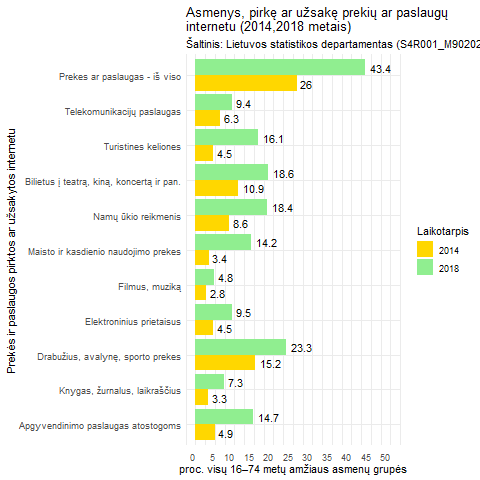
\includegraphics[scale=0.85]{Grafikai/2.png} 
\caption{Grafikas 4}
\label{fig:5}
\end{figure}
\medskip
Nagrinėjant Lietuvos statistikos departamento duomenis (žiūrėti lenetę nr. \ref{tab:4}) galima pastebėti, jog per 2015 - 2018 metų laikotarpiu, 2018 metais Lietuvos žmonės vis dažniau įsigydavo prekių ir paslaugų internetu. Jei 2015 metais prekių ir paslaugų 1-2 kartus įsigijusių žmonių skaičius buvo 52 procentai, tai 2018 metais jis sumažėjo 5.7 procento iki 46.3 procentų, tačiau apsipirkusių  3-5 kartus žmonių skaičius padidėjo nuo 33 iki 36 procentų, asmenų apsipirkusių 6-10 kartų skaičius išliko nepakitęs, o pirkėjų, pirkusių ar užsakiusių internetu daugiau nei 10 kartų skaičius išaugo nuo 4.3 iki 7 procentų. Galima daryti išvadą, jog Lietuvoje 2015-2018 metų laikotarpiu Lietuvos žmonės internetu apsipirkdavo dažniau ir daugiau.
\smallskip
\begin{table}[H]
\centering
\caption{Asmenys, pirkę ar užsakę prekių ar paslaugų internetu | proc.,kaip dažnai per paskutinius 3 mėn. internetu pirko visi 16-74 metų asmenys
Šaltinis: Lietuvos statistikos departamentas (S4R001\_M9020217)}
\label{tab:4}
\begin{tabular}{|l|l|l|}
\hline
Laikotarpis & Dažnumas per paskutinius 3 mėn. & Procentai \\ \hline
2015        & 1–2 kartus                      & 52.0      \\ \hline
2015        & 3–5 kartus                      & 33.0      \\ \hline
2015        & 6–10 kartų                      & 10.7      \\ \hline
2015        & daugiau kaip 10 kartų           & 4.3       \\ \hline
2018        & 1–2 kartus                      & 46.3      \\ \hline
2018        & 3–5 kartus                      & 36.0      \\ \hline
2018        & 6–10 kartų                      & 10.7      \\ \hline
2018        & daugiau kaip 10 kartų           & 7.0       \\ \hline
\end{tabular}
\end{table}
\smallskip
\par
Kaip pastebi \textcite{vsvcerbinskaite2018elektronines}, elektroninės prekybos plėtrai ir vystimuisi yra būtina palanki politinė sistema, šalies ekonominis išsivystymas ir informacinių technologijų tinklų paplitimas. Dėl laisvos interneto prieigos internetinės parduotuvės yra pasiekiamos lengviau todėl auga nuolatos internetu besinaudojančių žmonių skaičius ir tai sudaro sąlygas visuomenei dažniau apsipirkinėti elektroninėje erdvėje  ir elektroninės komercijos rinkai plėstis.
\smallskip
\begin{figure}[H]
\center
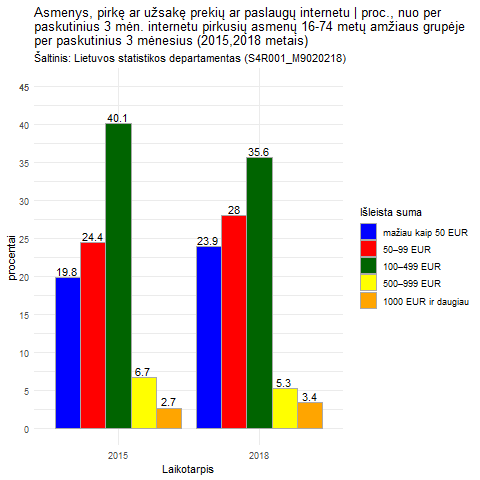
\includegraphics[scale=0.8]{Grafikai/6.png} 
\caption{Grafikas 5}
\label{fig:6}
\end{figure}
\medskip
\par
Lietuvos statistikos departamento duomenys (žiūrėti pav nr. \ref{fig:6}) iliustruoja, kaip Lietuvoje apsiperkant internetu išleidžiama pinigų suma skiriasi lyginant 2015 ir 2018 metus. Jei 2015 metais žmonių skaičius tarp visų 16-74 amžiaus žmonių, perkančių už mažiau kaip 50 EUR buvo 19.8 procento, tai 2018 metais šis rodiklis jau siekė 23.9 procentus ir indikuoja augimą. Asmenų, išledusių tarp 100 ir 499 EUR ir tarp 500 ir 999 EUR skaičius sumažėjo atitinkamai 4.5 ir 1.4 procento per 2015 - 2018 metų laikotarpį, tačiau pirkėjų, pirkusių ar užsakiusių už 50-99 EUR ir už 1000 EUR arba daugiau atitinkamai padidėjo 4.2 ir 0.7 procento šiuo laikotarpiu. Taigi, galima manyti, kad Lietuvoje elektroninei prekybai išleidžiamos sumos per 2015 - 2018 metų laikotarpį išaugo ir iš to galima daryti išvadą, jog internetinė prekyba plėtėsi ir turi tendencijas augti toliau.
\newpage
\section{Išvados}
\medskip
\par
\hspace{\parindent}
\begin{enumerate}
\item Elektroninė prekyba kaip reiškinys turi ir teigiamų ir neigiamų aspektų, kurie turi įtakos vartotų apsisprendimui įsigyti prekių ir paslaugų internetu. Svarbiausi šio reiškinio privalumai yra galimybė sutaupyti laiką apsipirkimui, galimybė pasirinkti ir palyginti prekę iš įvairaus asortimento ir sutaupyti pinigų. Tačiau perkant ar užsakant internetu nėra galimybės įvertinti prekės kokybės, galimos techninės problemos, susijusios su prekės ar paslaugos apmokėjimu, pristatymu ir ar grąžinimu. Taigi, galutinį sprendimą priima pats vartotojas, remdamasis savo asmenine patirtimi ir pasirinkdamas sau patogų būdą.
\item Lietuvoje 2014 - 2018 metais internetinė prekyba prekėmis ir paslaugomis plėtėsi. Internetinė prekyba išsaugo tarp visų amžiaus grupių ir didžiausią pirkėjų dalį sudarė jauni žmonės nuo 16 iki 34 metų. Apsipirkinėjimo dažnumas taip tad padidėjo ir 2018 metais Lietuvoje prekes ir paslaugas iš viso pirko arba užsakė 17.4 procentų daugiau asmenų nei 2014 metais.
\end{enumerate}
\newpage
\printbibliography[title={Literatūros sąrašas}]
\end{document}
